%!TEX root = ../my_thesis.tex
\section{The Large Hadron Collider}
\label{sec:lhc}

The \emph{Large Hadron Collider} (LHC) is a circular collider with a circumference of $26.66~\rm km$. It is located at CERN, near Geneva, between Switzerland and France.
The LHC is designed to produce proton-proton ($pp$) collisions with a \emph{luminosity} of $10^{34}~\rm cm^{-2}\rm s^{-1}$ and a centre-of-mass energy of $14~\rm TeV$.
In the first data-taking period before the first long shutdown, called Run 1 (2010--2012), the centre-of-mass energy reached $7~\rm TeV$ (2010--2011) and $8~\rm TeV$ (2012). 

The proton bunches, produced from hydrogen gas, pass through different intermediate accelerating stages (Fig.~\ref{fig:accelerators}):
\begin{itemize}[noitemsep,topsep=0pt]
	\item LINAC 2 ($50~\rm MeV$);
	\item Proton Synchroton Booster ($1.4~\rm GeV$);
	\item Proton Synchroton ($25~\rm GeV$);
	\item Super Proton Synchroton ($450~\rm GeV$).
\end{itemize}
Finally, they are injected clockwise and counter-clockwise into the LHC and accelerated to their final energy. 
Each bunch contains $\sim 10^{11}$ protons, and the nominal number of bunches per beam is 2808.
At LHC, in addition to LHCb, there are two general-purpose detectors (ATLAS and CMS), a detector dedicated to quark matter and quark-gluon plasma physics (ALICE) and other smaller experiments (TOTEM, LHCf, MoEDAL) dedicated to different topics.

\begin{figure}[htbp]
  \begin{center}
    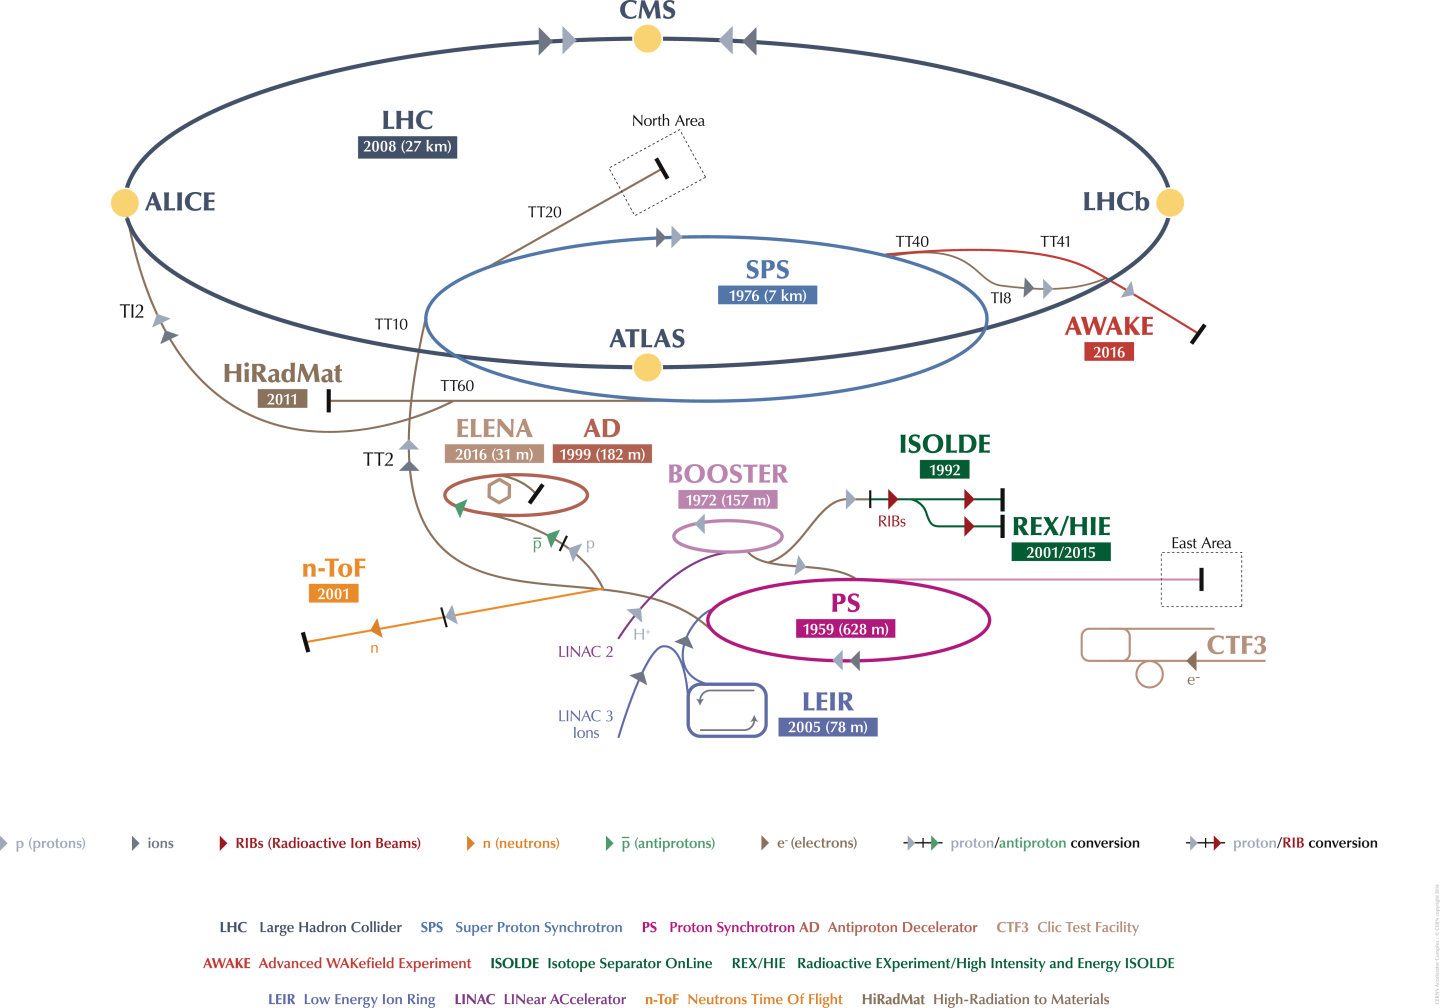
\includegraphics[width=1.1\textwidth]{01LHC/figs/accelerators.png}
  \end{center}
  \vspace{-2mm}
  \caption{Overview of the CERN accelerators complex.}
  \label{fig:accelerators}
\end{figure}

The LHC can also accelerate particles other than protons, such as lead or xenon nuclei, in order to collect data samples for specific studies.
